\subsection{関手の合成の関手化}\label{chap-7.3-functorization-of-functor-of-composite}
  射の合成は$\cat{Set}$の射\[\mor{\circ}{\arset{C}{B}{C}\times\arset{C}{A}{B}}{\arset{C}{A}{C}}\]で表される。これは小さい圏の圏$\cat{Cat}$でも当てはまり、\[\mor{\circ}{\arset{Cat}{\cat{B}}{\cat{C}}\times\arset{Cat}{\cat{A}}{\cat{B}}}{\arset{Cat}{\cat{A}}{\cat{C}}}\]となる。しかし現在では関手の集合である射集合よりも関手を対象に持つ関手圏が定義できている。そこで関手の合成に現れる射集合を関手圏に置き換えることはできないだろうか。
  すなわち、\[\functor{\circ}{\funccat{B}{C}\times\funccat{A}{B}}{\funccat{A}{C}}\]となるような関手を考えたい。対象関数については単に関手の合成で表せるが、射関数をどのように構成するかがこれからの議論の核となる。
  \begin{define}[自然変換と関手の合成]\label{def-composition-of-nat-and-functor}
    関手$\functor{F,G}{C}{D}$と自然変換$\nat{\alpha}{F}{G}$、関手$\functor{F'}{D}{E}$に対して、自然変換$\nat{F'\circ\alpha}{F'F}{F'G}$を$\cat{C}$の任意の対象$C$に対して$(F'\circ\alpha)_C=F'(\alpha_C)$と定義する。\\
    すなわち、圏$\cat{D}$の$\alpha$の成分を関手$F$の射関数で圏$\cat{E}$に写す。そして得られた$F(\alpha_C)$を自然変換の成分とみなす、という流れである。さてこれが実際に自然変換となることを示そう。\\
    まず$F(\alpha_A)$が圏$\cat{C}$の任意の対象$C$に対して存在することは、$\alpha_A$がそうであることと、関手$F'$が任意の射を何かしらの射へ写すことから分かる。よって後は自然性を示せば良い。だがこれは関手$F'$の合成の保存と$\alpha$の自然性によって簡単に示せる。
    \[F'\alpha_B\circ F'Ff=F'(\alpha_B\circ Ff)=F'(Gf\circ\alpha_A)=F'Gf\circ F'\alpha_A\]よって確かに自然変換である。
    \begin{center}
      \begin{tikzpicture}[auto]
        \node (A) at (-4, 5) {$A$};
        \node (B) at (-2, 5) {$B$};
        \node (FA) at (-1, 6) {$FA$};
        \node (FB) at (1, 6) {$FB$};
        \node (GA) at (-1, 4) {$GA$};
        \node (GB) at (1, 4) {$GB$};
        \node (F'FA) at (2, 6) {$F'FA$};
        \node (F'FB) at (4, 6) {$F'FB$};
        \node (F'GA) at (2, 4) {$F'GA$};
        \node (F'GB) at (4, 4) {$F'GB$};
        \node (catc) at (-3, 8) {$\cat{C}$};
        \node (catd) at (0, 8) {$\cat{D}$};
        \node (cate) at (3, 8) {$\cat{E}$};

        \draw[->] (A) to node{$f$}(B);

        \draw[->] (FA) to node{$Ff$}(FB);
        \draw[->] (GA) to node{$Gf$}(GB);
        \draw[->] (FA) to node{$\alpha_A$}(GA);
        \draw[->] (FB) to node{$\alpha_B$}(GB);

        \draw[->] (F'FA) to node{$F'Ff$}(F'FB);
        \draw[->] (F'GA) to node{$F'Gf$}(F'GB);
        \draw[->] (F'FA) to node{$F'(\alpha_A)$}(F'GA);
        \draw[->] (F'FB) to node{$F'(\alpha_B)$}(F'GB);
        \draw[->] (catd) to node{$F'$}(cate);

        \draw[->,bend left = 20] (catc) to node (funcf){$F$}(catd);
        \draw[->,bend right = 20] (catc) to node (funcg)[swap]{$G$}(catd);
        \draw[double,double equal sign distance,-implies,shorten >=5pt,shorten <=5pt] (funcf) -- node[label=right:$\alpha$] {} (funcg);
      \end{tikzpicture}
    \end{center}
    \begin{center}
      \begin{tikzpicture}[auto]
        \node (A) at (-4, 5) {$A$};
        \node (B) at (-2, 5) {$B$};
        \node (F'FA) at (-1, 6) {$F'FA$};
        \node (F'FB) at (1, 6) {$F'FB$};
        \node (F'GA) at (-1, 4) {$F'GA$};
        \node (F'GB) at (1, 4) {$F'GB$};
        \node (catc) at (-3, 8) {$\cat{C}$};
        \node (cate) at (0, 8) {$\cat{E}$};

        \draw[->] (A) to node{$f$}(B);

        \draw[->] (F'FA) to node{$F'Ff$}(F'FB);
        \draw[->] (F'GA) to node{$F'Gf$}(F'GB);
        \draw[->] (F'FA) to node{$(F'\circ\alpha)_A$}(F'GA);
        \draw[->] (F'FB) to node{$(F'\circ\alpha)_B$}(F'GB);
        \draw[->,bend left = 20] (catc) to node (funcf){$F'F$}(catd);
        \draw[->,bend right = 20] (catc) to node (funcg)[swap]{$F'G$}(cate);
        \draw[double,double equal sign distance,-implies,shorten >=5pt,shorten <=5pt] (funcf) -- node[label=right:$F'\circ\alpha$] {} (funcg);
      \end{tikzpicture}
    \end{center}
  \end{define}
  次に自然変換の後ろに関手を合成する操作を考えよう。
  \begin{define}[関手と自然変換の合成]\label{def-composition-of-functor-and-nat}
    関手$\functor{F',G'}{D}{E}$と自然変換$\nat{\beta}{F'}{G'}$、関手$\functor{F}{C}{D}$に対して自然変換$\nat{\beta\circ F}{F'F}{G'F}$を$\cat{C}$の任意の対象$C$に対して$(\beta\circ F)_C=\beta_{FC}$と定義する。これは自然変換$\beta$の量化の範囲を$F$で写された範囲に限定するという流れである。\\
    ここでの$\mor{\beta_{FC}}{F'FC}{G'FC}$は単に$\beta$の$FC$成分であるから自然性はすでに満たす。圏$\cat{C}$の任意の対象$C$に対して成分$\beta_{FC}$が存在するかどうかであるが、関手$F$は$C$を何らかの対象に写すため、$\beta_{FC}$は存在する。よって$\beta F$は自然変換である。
    \begin{center}
      \begin{tikzpicture}[auto]
        \node (A) at (-4, 5) {$A$};
        \node (B) at (-2, 5) {$B$};
        \node (FA) at (-1, 5) {$FA$};
        \node (FB) at (1, 5) {$FB$};
        \node (F'FA) at (2, 6) {$F'FA$};
        \node (F'FB) at (4, 6) {$F'FB$};
        \node (F'GA) at (2, 4) {$G'FA$};
        \node (F'GB) at (4, 4) {$G'FB$};
        \node (catc) at (-3, 8) {$\cat{C}$};
        \node (catd) at (0, 8) {$\cat{D}$};
        \node (cate) at (3, 8) {$\cat{E}$};

        \draw[->] (A) to node{$f$}(B);

        \draw[->] (FA) to node{$Ff$}(FB);

        \draw[->] (F'FA) to node{$F'Ff$}(F'FB);
        \draw[->] (F'GA) to node{$G'Ff$}(F'GB);
        \draw[->] (F'FA) to node{$\beta_{FA}$}(F'GA);
        \draw[->] (F'FB) to node{$\beta_{FB}$}(F'GB);
        \draw[->] (catc) to node{$F$}(catd);

        \draw[->,bend left = 20] (catd) to node (funcf){$F'$}(cate);
        \draw[->,bend right = 20] (catd) to node (funcg)[swap]{$G'$}(cate);
        \draw[double,double equal sign distance,-implies,shorten >=5pt,shorten <=5pt] (funcf) -- node[label=right:$\beta$] {} (funcg);
      \end{tikzpicture}
    \end{center}

    \begin{center}
      \begin{tikzpicture}[auto]
        \node (A) at (-4, 5) {$A$};
        \node (B) at (-2, 5) {$B$};
        \node (F'FA) at (-1, 6) {$F'FA$};
        \node (F'FB) at (1, 6) {$F'FB$};
        \node (F'GA) at (-1, 4) {$G'FA$};
        \node (F'GB) at (1, 4) {$G'FB$};
        \node (catc) at (-3, 8) {$\cat{C}$};
        \node (cate) at (0, 8) {$\cat{E}$};
  
        \draw[->] (A) to node{$f$}(B);
  
        \draw[->] (F'FA) to node{$F'Ff$}(F'FB);
        \draw[->] (F'GA) to node{$G'Ff$}(F'GB);
        \draw[->] (F'FA) to node{$(\beta\circ F)_A$}(F'GA);
        \draw[->] (F'FB) to node{$(\beta\circ F)_B$}(F'GB);
  
        \draw[->,bend left = 20] (catc) to node (funcf){$F'F$}(cate);
        \draw[->,bend right = 20] (catc) to node (funcg)[swap]{$G'F$}(cate);
        \draw[double,double equal sign distance,-implies,shorten >=5pt,shorten <=5pt] (funcf) -- node[label=right:$\beta\circ F$] {} (funcg);
      \end{tikzpicture}
    \end{center}
  \end{define}
  次にいよいよ合成を行う関手の射関数となるような操作を定義する。またこの合成は関手圏における射の合成である垂直合成と区別するため水平合成と呼ぶことにする。
  \begin{define}[自然変換の水平合成]\label{def-horizonal-compositon-of-natural-transfomations}
    関手$\functor{F,G}{C}{D},\ \functor{F',G'}{D}{E}$と自然変換$\nat{\alpha}{F}{G},\ \nat{\beta}{F'}{G'}$に対して\textbf{垂直合成}された自然変換$\nat{\beta\alpha}{F'F}{G'G}$を\[\beta\circ\alpha = \alpha G'\cdot F\beta = G\beta\cdot\alpha F'\]とする。\\
    \begin{center}
      \begin{tikzpicture}[auto]
        \node (cat) at (1, 1) {$\funccat{C}{E}$};
        \node (FF) at (0, 0) {$F'F$};
        \node (FG) at (2, 0) {$F'G$};
        \node (GF) at (0, -2) {$G'F$};
        \node (GG) at (2, -2) {$G'G$};
        \draw[double,double equal sign distance,-implies] (FF) to node{$\beta\circ F$}(GF);
        \draw[double,double equal sign distance,-implies] (FG) to node{$\beta\circ G$}(GG);
        \draw[double,double equal sign distance,-implies] (FF) to node{$F'\circ\alpha$}(FG);
        \draw[double,double equal sign distance,-implies] (GF) to node{$G'\circ\beta$}(GG);
      \end{tikzpicture}
    \end{center}
    成分を見ると、$\cat{C}$の任意の対象$C$に対して成分\[(\beta\circ\alpha)_C=G'\alpha_C\circ \beta_{FC}=\beta_{GC}\circ F'\alpha_C\]となる。
    自然変換と関手の合成と関手の自然変換の合成をそれぞれ用いて定義されているが、これらが自然変換であることはすでに示した。よってその二つを合成した$\beta\circ\alpha$も自然変換である。\\
    さて自然変換の水平合成の直感を得るためにも$\alpha G'\cdot F\beta = G\beta\cdot\alpha F'$を示そう。これは上に書いたように$A$に対して成分の等式\[G'\alpha_A\circ \beta_{FA}=\beta_{GA}\circ F'\alpha_A\]が成り立てば良い。
    \begin{center}
      \begin{tikzpicture}[auto]
        \node (A) at (-2, 5) {$A$};
        \node (FA) at (0, 6) {$FA$};
        \node (GA) at (0, 4) {$GA$};
        \node (F'FA) at (2, 6) {$F'FA$};
        \node (F'FB) at (4, 6) {$G'FA$};
        \node (F'GA) at (2, 4) {$F'GA$};
        \node (F'GB) at (4, 4) {$G'GA$};
        \node (catc) at (-2, 8) {$\cat{C}$};
        \node (catd) at (0, 8) {$\cat{D}$};
        \node (cate) at (3, 8) {$\cat{E}$};


        \draw[->] (FA) to node{$\alpha_A$}(GA);

        \draw[->] (F'FA) to node{$\beta_{FA}$}(F'FB);
        \draw[->] (F'GA) to node{$\beta_{GA}$}(F'GB);
        \draw[->] (F'FA) to node{$F'\alpha_A$}(F'GA);
        \draw[->] (F'FB) to node{$G'\alpha_A$}(F'GB);


        \draw[->,bend left = 20] (catd) to node (funcf'){$F'$}(cate);
        \draw[->,bend right = 20] (catd) to node (funcg')[swap]{$G'$}(cate);
        \draw[->,bend left = 30] (catc) to node (funcf){$F$}(catd);
        \draw[->,bend right =30] (catc) to node (funcg)[swap]{$G$}(catd);
        \draw[double,double equal sign distance,-implies,shorten >=5pt,shorten <=5pt] (funcf) -- node[label=right:$\alpha$] {} (funcg);
        \draw[double,double equal sign distance,-implies,shorten >=5pt,shorten <=5pt] (funcf') -- node[label=right:$\beta$] {} (funcg');
      \end{tikzpicture}
    \end{center}
    ここで$FA=B,\ GA=C, \alpha_A=f$と置くと、これは明らかに$\beta$の自然性であり成り立つ。
    \begin{center}
      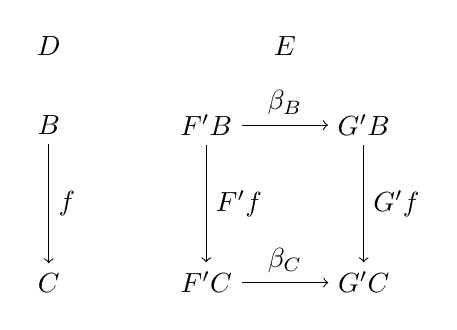
\begin{tikzpicture}[auto]
        \node (FA) at (0, 6) {$B$};
        \node (GA) at (0, 4) {$C$};
        \node (F'FA) at (2, 6) {$F'B$};
        \node (F'FB) at (4, 6) {$G'B$};
        \node (F'GA) at (2, 4) {$F'C$};
        \node (F'GB) at (4, 4) {$G'C$};
        \node (catd) at (0, 7) {$\cat{D}$};
        \node (cate) at (3, 7) {$\cat{E}$};
        \draw[->] (FA) to node{$f$}(GA);

        \draw[->] (F'FA) to node{$\beta_{B}$}(F'FB);
        \draw[->] (F'GA) to node{$\beta_{C}$}(F'GB);
        \draw[->] (F'FA) to node{$F'f$}(F'GA);
        \draw[->] (F'FB) to node{$G'f$}(F'GB);
      \end{tikzpicture}
    \end{center}
  \end{define}
  また、$\alpha$を恒等自然変換とすると関手と自然変換の合成になり、$\beta$を恒等自然変換とすると自然変換と関手の合成になる。よってどちらも自然変換の水平合成と呼ぶことにする。
  \begin{define}[関手を合成する関手]\label{def-functor-composite-functors}
    関手を合成する関手$\functor{\circ}{\funccat{D}{E}\times \funccat{C}{D}}{\funccat{C}{E}}$を以下のように定義する。
    \begin{quote}
			\begin{mydescription}
		\item[対象関数]対象関数
    \[\functor{\circ}{\obj{\funccat{D}{E}\times\funccat{C}{D}}}{\obj{\funccat{C}{E}}}\]は、積圏の対象の集合の定義より、\[\functor{\circ}{\obj{\funccat{D}{E}}\times\obj{\funccat{C}{D}}}{\obj{\funccat{C}{E}}}\]と表せる。また関手圏の対象集合の定義より、\[\mor{\circ}{\arset{Cat}{\cat{D}}{\cat{E}}\times\arset{Cat}{\cat{C}}{\cat{D}}}{\arset{Cat}{\cat{C}}{\cat{E}}}\]とも表せるから、$\cat{Cat}$の定義に用いられる関手の合成を対象関数とする。
		\item[射関数]任意の関手$\functor{F,G}{C}{D},\ \functor{F',G'}{D}{E}$に対する射関数\[\mor{\circ}{\arset{\funccat{D}{E}\times\funccat{C}{D}}{\tuple{F',F}}{\tuple{G',G}}}{\arset{\funccat{C}{E}}{F'\circ F}{G'\circ G}}\]を任意の自然変換$\nat{\alpha}{F}{G},\ \nat{\beta}{F'}{G'}$に対して
    \[\circ(\beta,\alpha)=\beta\circ\alpha\]と定義する。
    \begin{center}
      \begin{tikzpicture}[auto]
        \node (cata) at (0, 1) {$\funccat{D}{E}\times\funccat{C}{D}$};
        \node (cata) at (2, 1) {$\funccat{C}{E}$};
        \node (F'F) at (0, 0) {$\tuple{F',F}$};
        \node (G'G) at (0, -2) {$\tuple{G',G}$};
        \draw[->] (F'F) to node{$\tuple{\beta,\alpha}$}(G'G);
        \node (F'cF) at (2, 0) {$F'\circ F$};
        \node (G'cG) at (2, -2) {$G'\circ G$};
        \draw[double,double equal sign distance,-implies] (F'cF) to node{$\beta\circ\alpha$}(G'cG);
        \draw[-,dashed] (F'F) to (F'cF);
        \draw[-,dashed] (G'G) to (G'cG);

      \end{tikzpicture}
    \end{center}
		\item[恒等射の保存]積圏の恒等射の定義より、$\tuple{F',F}$の恒等射は$\nat{\tuple{ID_{F'},ID_{F}}}{\tuple{F',F}}{\tuple{F',F}}$であるから、$ID_{F'}\circ ID_{F}=ID_{F'F}$を示せば良い。これは$\cat{C}$の任意の対象$C$おいて
    \begin{align*}
      (ID_{F'}\circ ID_F)_C &= F'(ID_{F})_C\circ (ID_{F'})_{FC}&\text{(自然変換の水平合成)}\\
      &=F'(id_{FC})\circ id_{F'FC}&\text{(恒等自然変換の定義)}\\
      &=id_{F'FC}\circ id_{F'FC}&\text{(関手の恒等射の保存)}\\
      &=id_{F'FC}
    \end{align*}
    となるから$ID_{F'}\circ ID_{F}=ID_{F'F}$である。
		\item[射の合成の保存]任意の$\functor{F,G,H}{C}{D},\ \functor{F',G',H'}{D}{E}$と自然変換$\nat{\alpha}{F}{G},\ \nat{\beta}{F'}{G'},\ \nat{\alpha'}{G}{H},\ \nat{\beta'}{G'}{H'}$に対して
    \[(\beta'\cdot\beta)\circ(\alpha'\cdot\alpha)=(\beta'\circ\alpha')\cdot(\beta\circ\alpha)\]が成り立つことを示せば良い。
    \begin{center}
      \begin{tikzpicture}[auto]
        \node (catc) at (-3, 8) {$\cat{C}$};
        \node (catd) at (0, 8) {$\cat{D}$};
        \node (cate) at (3, 8) {$\cat{E}$};
        \draw[->,bend left = 40] (catd) to node (funcf'){$F'$}(cate);
        \draw[->] (catd) to node[yshift =-7,fill=white] (funcg'){$G'$}(cate);
        \draw[->,bend right = 40] (catd) to node (funch')[swap]{$H'$}(cate);

        \draw[->,bend left = 40] (catc) to node (funcf){$F$}(catd);
        \draw[->] (catc) to node[yshift =-7,fill=white] (funcg){$G$}(catd);
        \draw[->,bend right =40] (catc) to node (funch)[swap]{$H$}(catd);
        \draw[double,double equal sign distance,-implies,shorten >=0pt,shorten <=2pt] (funcf) -- node[label=right:$\alpha$] {} (funcg);
        \draw[double,double equal sign distance,-implies,shorten >=0pt,shorten <=2pt] (funcf') -- node[label=right:$\beta$] {} (funcg');
        \draw[double,double equal sign distance,-implies,shorten >=2pt,shorten <=0pt] (funcg) -- node[label=right:$\alpha'$] {} (funch);
        \draw[double,double equal sign distance,-implies,shorten >=2pt,shorten <=0pt] (funcg') -- node[label=right:$\beta'$] {} (funch');
      \end{tikzpicture}
    \end{center}
		圏$\cat{C}$の任意の対象$A$に対して、
    \begin{align*}
      ((\beta'\cdot\beta)\circ(\alpha'\cdot\alpha))_A&=H'(\alpha'\cdot\alpha)_A\circ(\beta'\cdot\beta)_{FA}&\text{(水平合成の定義)}\\
      &=H'\alpha'_A\circ H'\alpha_A\circ\beta'_{FA}\circ\beta_{FA}&\text{(垂直合成の定義)}\\
      &=H'\alpha'_A\circ\beta'_{GA}\circ G'\alpha_A\circ\beta_{FA}&\text{($\beta$の自然性)}\\
      &=(\beta'\circ\alpha')_A\circ(\beta\circ\alpha)_A&\text{(水平合成の定義)}\\
      &=((\beta'\circ\alpha')\cdot(\beta\circ\alpha))_A&\text{(垂直合成の定義)}
    \end{align*}
    \begin{center}
      \begin{tikzpicture}[auto]
        \node (cata) at (0, 1) {$\funccat{D}{E}\times\funccat{C}{D}$};
        \node (cata) at (2, 1) {$\funccat{C}{E}$};
        \node (F'F) at (0, 0) {$\tuple{F',F}$};
        \node (G'G) at (0, -2) {$\tuple{G',G}$};
        \node (H'H) at (0, -4) {$\tuple{H',H}$};

        \draw[->] (F'F) to node[swap]{$\tuple{\beta,\alpha}$}(G'G);
        \draw[->] (G'G) to node[swap]{$\tuple{\beta',\alpha'}$}(H'H);

        \node (F'cF) at (2, 0) {$F'\circ F$};
        \node (G'cG) at (2, -2) {$G'\circ G$};
        \node (H'cH) at (2, -4) {$H'\circ H$};

        \draw[double,double equal sign distance,-implies] (F'cF) to node[swap]{$\beta\circ\alpha$}(G'cG);
        \draw[double,double equal sign distance,-implies] (G'cG) to node[swap]{$\beta'\circ\alpha'$}(H'cH);
        \draw[double,double equal sign distance,-implies,bend left = 30] (F'cF) to node{$(\beta'\cdot\beta)\circ(\alpha'\cdot\alpha)$}(H'cH);
        \draw[-,dashed] (F'F) to (F'cF);
        \draw[-,dashed] (G'G) to (G'cG);
        \draw[-,dashed] (H'H) to (H'cH);

      \end{tikzpicture}
    \end{center}
    よって$(\beta'\cdot\beta)\circ(\alpha'\cdot\alpha)=(\beta'\circ\alpha')\cdot(\beta\circ\alpha)$である。またこの性質を相互交換法則と呼ぶことにする。
		\end{mydescription}
		\end{quote}
  \end{define}
  関手の合成を関手として定義できたわけだが、これを$\cat{Cat}$における射の合成の代わりに使用できるかと考えるが、それを行うには圏の定義から考え直さなくてはいけなくなる。現時点で触れる予定は無いが、興味がある場合は2-Categoryに関する文献を読むと良い。\\
  また関手の同型の保存より以下の命題がすぐに成り立つ。
  \begin{prop}[関手合成の同型の保存]\label{prop-preservation-of-isomorphism-by-composition-functors}
    関手$\functor{F,F'}{C}{D},\ \functor{G,G'}{D}{E}$に対して$F\cong F',\ G\cong G'\Longrightarrow G\circ F\cong G'\circ F'$
  \end{prop}
  \begin{proof}
    双関手の同型の保存より\[F\cong F',\ G\cong G'\Longrightarrow\tuple{G,F}\cong\tuple{G',F'}\]\\
    また関手を合成する関手の同型の保存より、\[\tuple{G,F}\cong\tuple{G',F'}\Longrightarrow G\circ F\cong G'\circ F'\]
    よって$F\cong F',\ G\cong G'\Longrightarrow G\circ F\cong G'\circ F'$が成り立つ。
  \end{proof}
  さて、自然変換の水平合成や相互交換法則に触れた理由として、関手圏やその合成を行う関手の性質によって、関手や自然変換の満たすべき性質を復元できるからである。特に関手の合成の保存や、自然性などは仮定する動機が不十分であったから、これらを$\cat{Cat}$の持つ性質と見なして改めて導出しよう。\\


    自然性と水平合成の関係を見る。一点離散圏$\cat{1}$と任意の圏$\cat{C,D}$、関手$\functor{A,B}{1}{C},\ \functor{F,G}{C}{D}$、自然変換$\nat{f}{A}{B},\ \nat{\alpha}{F}{G}$を考える。
    \begin{center}
      \begin{tikzpicture}[auto]
        \node (*) at (-2, 5) {$*$};
        \node (A) at (0, 6) {$A*$};
        \node (B) at (0, 4) {$B*$};
        \node (FA) at (2, 6) {$FA*$};
        \node (GA) at (4, 6) {$GA*$};
        \node (FB) at (2, 4) {$FB*$};
        \node (GB) at (4, 4) {$GB*$};
        \node (cat1) at (-2, 8) {$\cat{1}$};
        \node (catc) at (0, 8) {$\cat{C}$};
        \node (catd) at (3, 8) {$\cat{D}$};


        \draw[->] (A) to node{$f_*$}(B);

        \draw[->] (F'FA) to node{$\alpha_{A*}$}(F'FB);
        \draw[->] (F'GA) to node{$\alpha_{B*}$}(F'GB);
        \draw[->] (F'FA) to node{$Ff_*$}(F'GA);
        \draw[->] (F'FB) to node{$Gf_*$}(F'GB);

        \draw[->,bend left = 30] (cat1) to node (funcf'){$A$}(catc);
        \draw[->,bend right = 30] (cat1) to node (funcg')[swap]{$B$}(catc);
        \draw[->,bend left = 20] (catc) to node (funcf){$F$}(catd);
        \draw[->,bend right =20] (catc) to node (funcg)[swap]{$G$}(catd);
        \draw[double,double equal sign distance,-implies,shorten >=5pt,shorten <=5pt] (funcf) -- node[label=right:$\alpha$] {} (funcg);
        \draw[double,double equal sign distance,-implies,shorten >=5pt,shorten <=5pt] (funcf') -- node[label=right:$f$] {} (funcg');
      \end{tikzpicture}
    \end{center}
    $A=A(*),\ B=B(*),\ f=f_*$とすると、以下のような図式が書ける。
    \begin{center}
      \begin{tikzpicture}[auto]
        \node (*) at (-2, 5) {$*$};
        \node (A) at (0, 6) {$A$};
        \node (B) at (0, 4) {$B$};
        \node (FA) at (2, 6) {$FA$};
        \node (GA) at (4, 6) {$GA$};
        \node (FB) at (2, 4) {$FB$};
        \node (GB) at (4, 4) {$GB$};
        \node (cat1) at (-2, 8) {$\cat{1}$};
        \node (catc) at (0, 8) {$\cat{C}$};
        \node (catd) at (3, 8) {$\cat{D}$};


        \draw[->] (A) to node{$f$}(B);

        \draw[->] (F'FA) to node{$\alpha_A$}(F'FB);
        \draw[->] (F'GA) to node{$\alpha_B$}(F'GB);
        \draw[->] (F'FA) to node{$Ff$}(F'GA);
        \draw[->] (F'FB) to node{$Gf$}(F'GB);


        \draw[->,bend left = 30] (cat1) to node (funcf'){$A$}(catc);
        \draw[->,bend right = 30] (cat1) to node (funcg')[swap]{$B$}(catc);
        \draw[->,bend left = 20] (catc) to node (funcf){$F$}(catd);
        \draw[->,bend right =20] (catc) to node (funcg)[swap]{$G$}(catd);
        \draw[double,double equal sign distance,-implies,shorten >=5pt,shorten <=5pt] (funcf) -- node[label=right:$\alpha$] {} (funcg);
        \draw[double,double equal sign distance,-implies,shorten >=5pt,shorten <=5pt] (funcf') -- node[label=right:$f$] {} (funcg');
      \end{tikzpicture}
    \end{center}
    これは任意の射、任意の対象で成り立つから、明らかに自然変換の図式である。\\

    関手の合成の保存と相互交換法則の関係性を見る。一点離散圏$\cat{1}$と任意の圏$\cat{C,D}$、関手$\functor{A,B,C}{1}{C},\ \functor{F}{C}{D}$、自然変換$\nat{f}{A}{B},\ \nat{g}{B}{C}$を考えると、相互交換法則より\[(ID_F\cdot ID_F)\circ(g\cdot f)=(ID_F\circ g)\cdot(ID_F\circ f)\]が成り立つ。この自然変換の$*$成分を取ると、
    \begin{align*}
      ((ID_F\cdot ID_F)\circ(g\cdot f))_*&=F(g\cdot f)_*\circ(ID_F\cdot ID_F)_{C*}&\text{(水平合成の定義)}\\
      &=F(g\cdot f)_*&\text{(恒等自然変換の定義)}\\
      ((ID_F\circ g)\cdot(ID_F\circ f))_*&=(ID_F\circ g)_*\circ(ID_F\circ f)_*&\text{(垂直合成の定義)}\\
      &=Fg_*\circ Ff_*&\text{(水平合成の定義)}\\
    \end{align*}
    となり、$f_*=f,\ g_*=g$とすると、$(g\cdot f)_*=g\circ f$であるから、
    この等式は$F(g\circ f)=Fg\circ Ff$と変形できる。
    \begin{center}
      \begin{tikzpicture}[auto]
        \node (catc) at (-3, 8) {$\cat{1}$};
        \node (catd) at (0, 8) {$\cat{C}$};
        \node (cate) at (3, 8) {$\cat{D}$};
        \draw[->,bend left = 40] (catd) to node (funcf'){$F$}(cate);
        \draw[->] (catd) to node[yshift =-7,fill=white] (funcg'){$F$}(cate);
        \draw[->,bend right = 40] (catd) to node (funch')[swap]{$F$}(cate);

        \draw[->,bend left = 40] (catc) to node (funcf){$A$}(catd);
        \draw[->] (catc) to node[yshift =-7,fill=white] (funcg){$B$}(catd);
        \draw[->,bend right =40] (catc) to node (funch)[swap]{$C$}(catd);
        \draw[double,double equal sign distance,-implies,shorten >=0pt,shorten <=2pt] (funcf) -- node[label=right:$f$] {} (funcg);
        \draw[double,double equal sign distance,-implies,shorten >=0pt,shorten <=2pt] (funcf') -- node[label=right:$ID_F$] {} (funcg');
        \draw[double,double equal sign distance,-implies,shorten >=2pt,shorten <=0pt] (funcg) -- node[label=right:$g$] {} (funch);
        \draw[double,double equal sign distance,-implies,shorten >=2pt,shorten <=0pt] (funcg') -- node[label=right:$ID_F$] {} (funch');
    \end{tikzpicture}
  \end{center}